\section{Introduction}\label{ch:intro}

Angry Birds is a succesfull video game. Goal of the game is destroying all the pigs in a given scene by shooting with different types of birds from a slingshot. You get points by destroying pigs and object structures like ice-blocks, stone-blocks or wooden-blocks\footnote{https://www.giga.de/apps/angry-birds-2/specials/angry-birds-2-vogelauswahl-faehigkeiten-strategietipps/}. For humans Angry Birds is easy to learn, understand and play. As a human it is ordinary to understand what will happen by shooting at a given structure because of the physical common knowledge. In contrast these tasks are difficult to capture for Artificial Intelligence. The use of Artificial Intelligence in games achieved progress. For example in the games Chess, Go, Poker or Arcade the AI agent is better than a human. But for some other strategy games, like Angry Birds, there is missing specific knowledge. 
Analysing the stability of structures with different force effects or physical common knowledge belongs to the missing knowledge. Further challenges are the image processing which has to recognise varying backgrounds and obstacles or the planning with insecurity because of the unknown physical proberties. A competition was launched to enhance the skills of Artificial Intelligence in strategy games,  like Angry Birds.
The AIBirds Competetition is the basis of our project and our agent. As foundation there was a game playing software including a computer vision module, a game interface that interacts with a Chrome version and a trajectory planning module. 
Goal of the competition is getting better with an intellgient Angry Birds-Agent than the best human players\footnote{https://aibirds.org/}.
The following chapters reflect our progress during the project and is split into the specific topics: 
We made a progress in the topic 'level editor' by using an already existing leveleditor. Now we can parse these levels in the corresponding file format for our agent. With that innovation it is possible to test our agent with more recent levels instead of the given levels of the competition.  There is also a random levelgenerator which can create different kinds of levels, like a Dominolevel, Houselevel or Funnellevel. The Evaluation chapter describes the implementation of a new evaluation framework which is time-saving and gives a structured overview of the performance of the compared agents. The chapter Shot Prediction focusses on trajectory estimation, which considers all bird types and and goes beyond the \ang{75} mark. We also implemented a new slingshot detection and a parabola evaluation after the shot. 
Another important aspect are the strategy improvements. To improve the strategy of the agent a decision tree was implemented. By loosing a level the agent saves the used strategy that lead to the failure. When the level gets restarted the agent tries a new strategy and also gains knowledge about whether a shot led to failure or pass of a level. Another part of the strategy chapter is machine learning.
We used 'Weka' - a collection of algorithms for machine learning.
The Miscellaneous chapter contains all topics which cannot be grouped into a category like the logger class or the code documentation with doxygen. In order to save time we implemented a logger class for text outputs to save cpu time.
A clear code documentation is necessary for a software project of this scope. The tool 'Doxygen' can be used for this. 
\begin{figure}
	\centering
	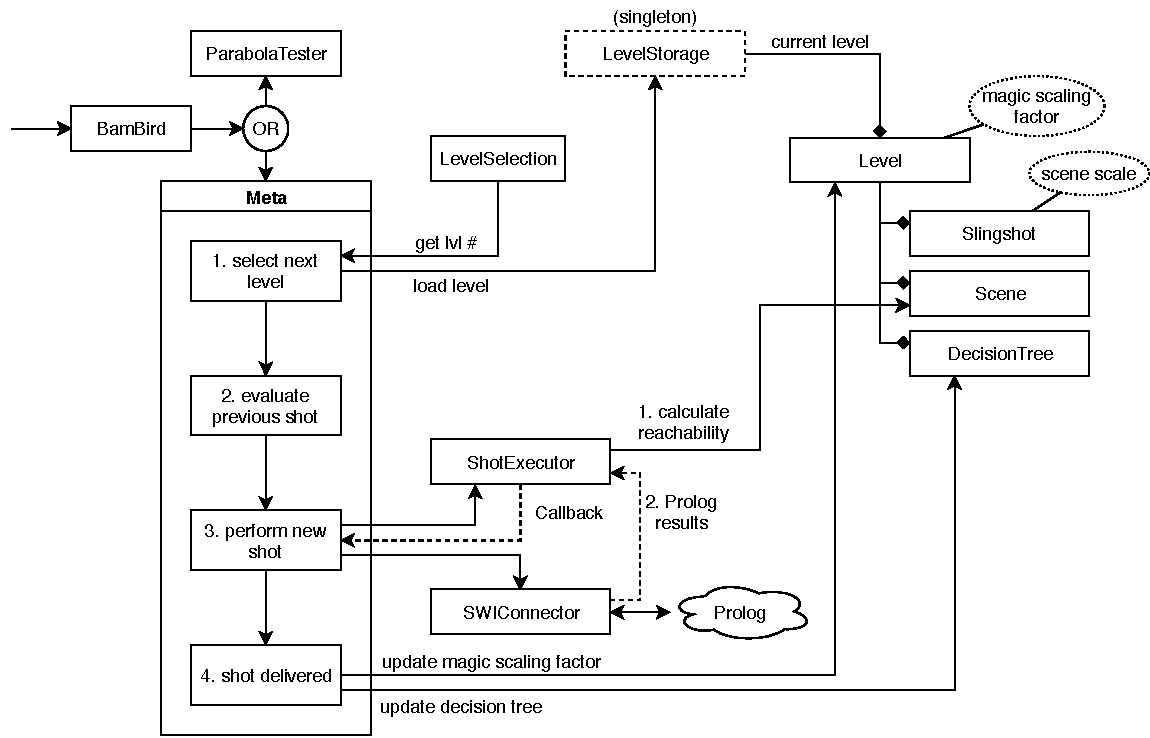
\includegraphics[width=\textwidth]{img/diagram-classes}
	\caption{Simplified main execution flow. From game initialization, to level selection and shot execution.}
	\label{img:intro:classes}
\end{figure}

\begin{figure}
	\centering
	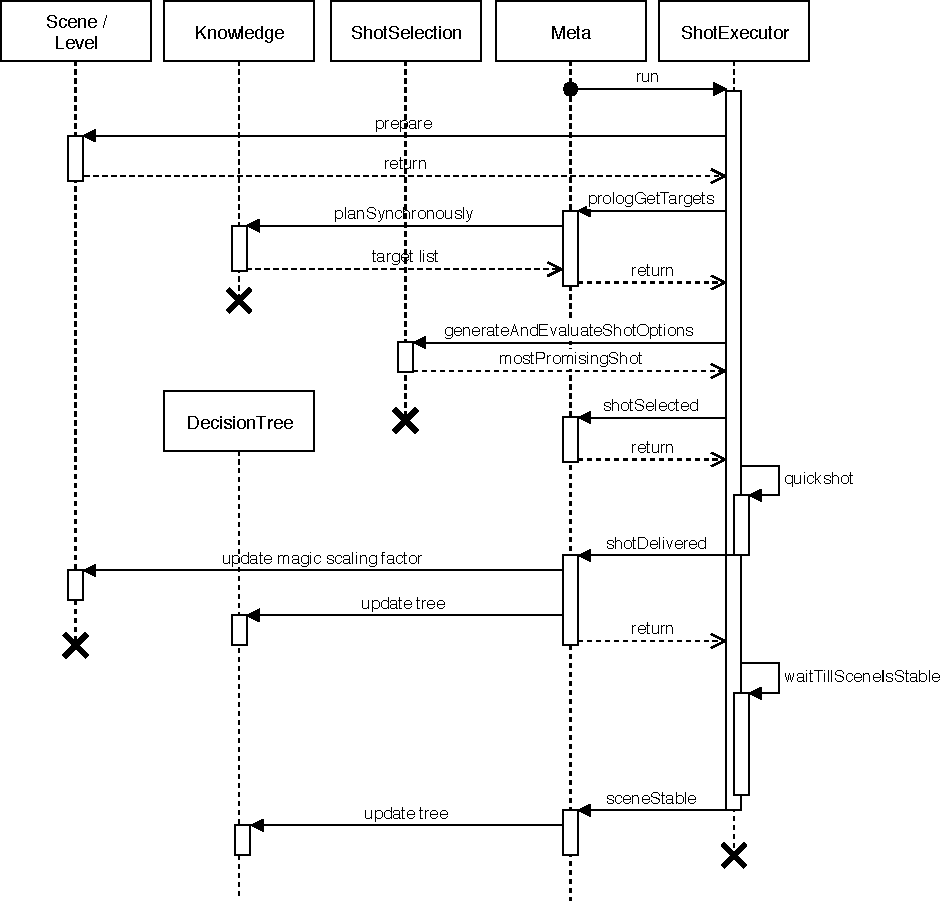
\includegraphics[width=\textwidth]{img/diagram-shotexecuter}
	\caption{Control flow for ShotExecutor class. Chart entry is Meta.}
	\label{img:intro:shotexecuter}
\end{figure}
